\documentclass[12pt, a4paper]{article}
\usepackage[utf8]{inputenc}
\usepackage{graphicx}
\graphicspath{ {img/} }

\title{First document}
\author{PIN-CHUN, HSU}
\date{April 2017}
\begin{document}

\maketitle

First document. This is a simple example, with no
extra parameters or packages included. %comment here
try

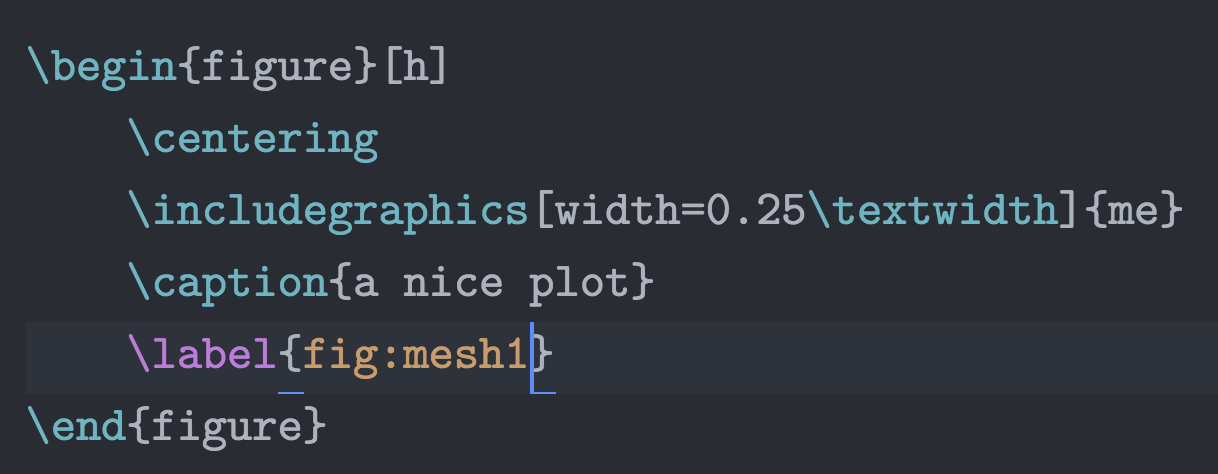
\includegraphics[width=50mm,scale=0.5]{tmp}

test
Some of \textbf{Bold texts}
and some \underline{Underline texts}
and more \textbf{\textit{Text it}}
\textbf{ already in bold font but still can \emph{Emphasize} something}

\begin{figure}[h]
    \centering
    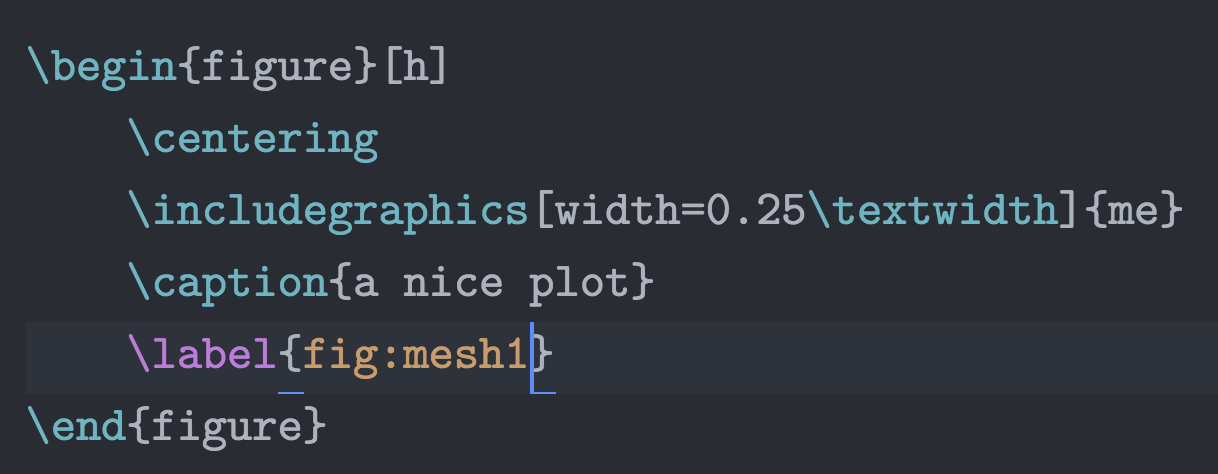
\includegraphics[width=0.25\textwidth]{tmp}
    \caption{a nice plot}
    \label{fig:mesh1}
\end{figure}

As you can see in the figure \ref{fig:mesh1}, the
function grows near 0. Also, in the page \pageref{fig:mesh1}
is the same example.

\end{document}
